\subsection{Glyph: \glyph{And}}
\label{sec:af:and}

The glyph \glyph{and} is used to denote that all the \glyph{ANs} linked as input are necessary to influence the target activity.

\begin{glyphDescription}
 \glyphSboTerm SBO:0000173 ! and.
 \glyphOrigin More than one \glyph{AN} (\sect{af:ANs}) and \glyph{logical arcs} (section~\ref{sec:af:logicArc}).
 \glyphTarget  \glyph{Modulation arc} (\sect{af:arcs}) other than \glyph{equivalence arc}.
 \glyphNode \glyph{And} is represented by a circle carrying the word ``AND'',  with two connectors located at the opposite side for inputs and output.
\end{glyphDescription}

\begin{figure}[H]
  \centering
  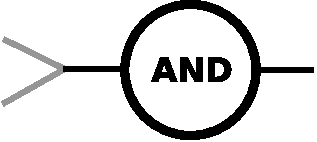
\includegraphics[scale = 0.5]{images/and}
  \caption{The \AF glyph for \glyph{and}. Only two inputs are represented, but more would be allowed.}
  \label{fig:af:and}
\end{figure}
